\documentclass{beamer}

\title{Exploring Semantic Hierarchies to Improve Resolution Theorem Proving on Ontologies}
\subtitle{Stanley C. Small}

\begin{document}
	\frame {
		\titlepage
	}
	
	\frame {
    	\frametitle{Agenda}
	Defense (2.5 Hours)
    	\begin{itemize}
		    \item Honors Thesis (1 Hour)
		    \begin{itemize}
     \item Presentation (20 min)
     \item Questions (40 min) 
   \end{itemize}
	        \item Honors Reading List (1 Hour)
	        		    \begin{itemize}
     \item Reading List Description (5 min)
     \item Reading List Discussion (55 min) 
   \end{itemize}
   \item Committee Deliberation (30 min)
    \begin{itemize}
     \item    Level of honors discussion
     \item Suggestions for Revision
   \end{itemize}
        \end{itemize}
	}
	
		    \frame{
	    \frametitle{Ontologies}
	    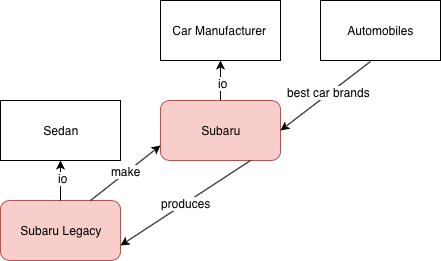
\includegraphics[width = \textwidth]{images/sample_ontology.png}
	}
	
			    \frame{
	    \frametitle{Theorem Proving}
	    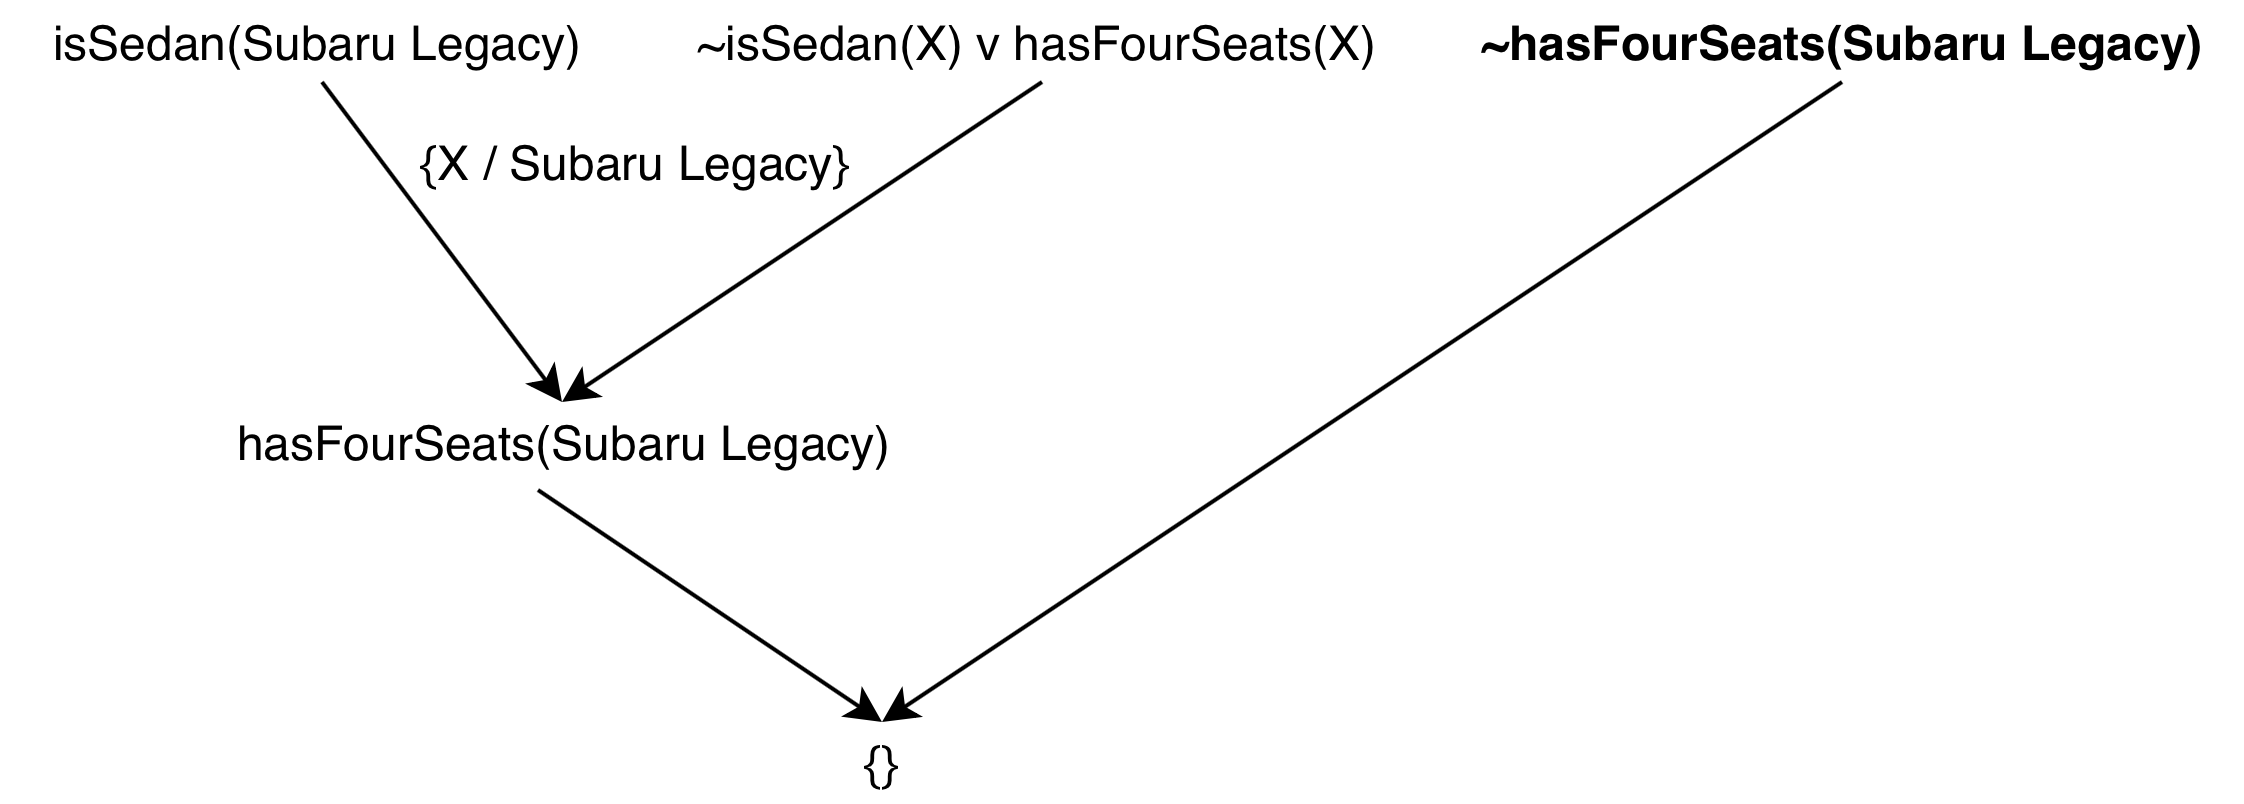
\includegraphics[width = \textwidth]{images/resolution_tree.png}
	}
	
	 \frame{
	    \frametitle{Semantic Heirarchies}
	    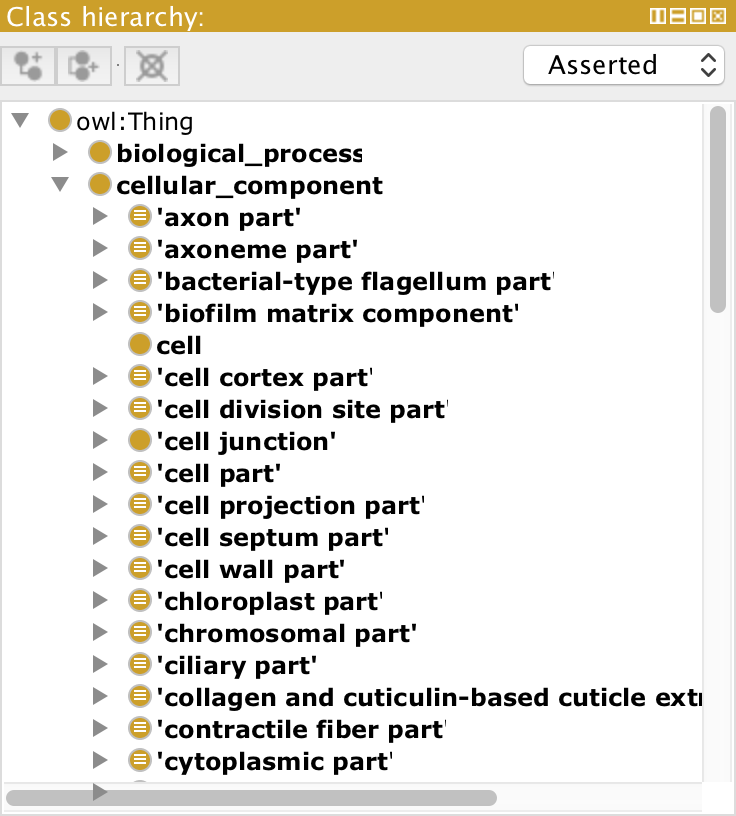
\includegraphics[width = 0.49\textwidth]{images/class-hierarchy.png}
	    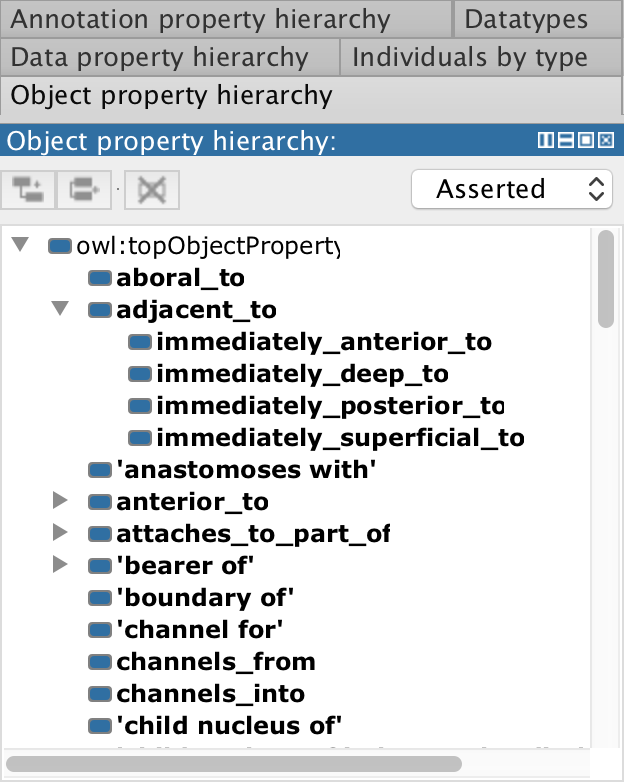
\includegraphics[width = 0.49\textwidth]{images/object-property-hierarchy.png}
	}
	
	    \frame{
	    \frametitle{Approach}
	    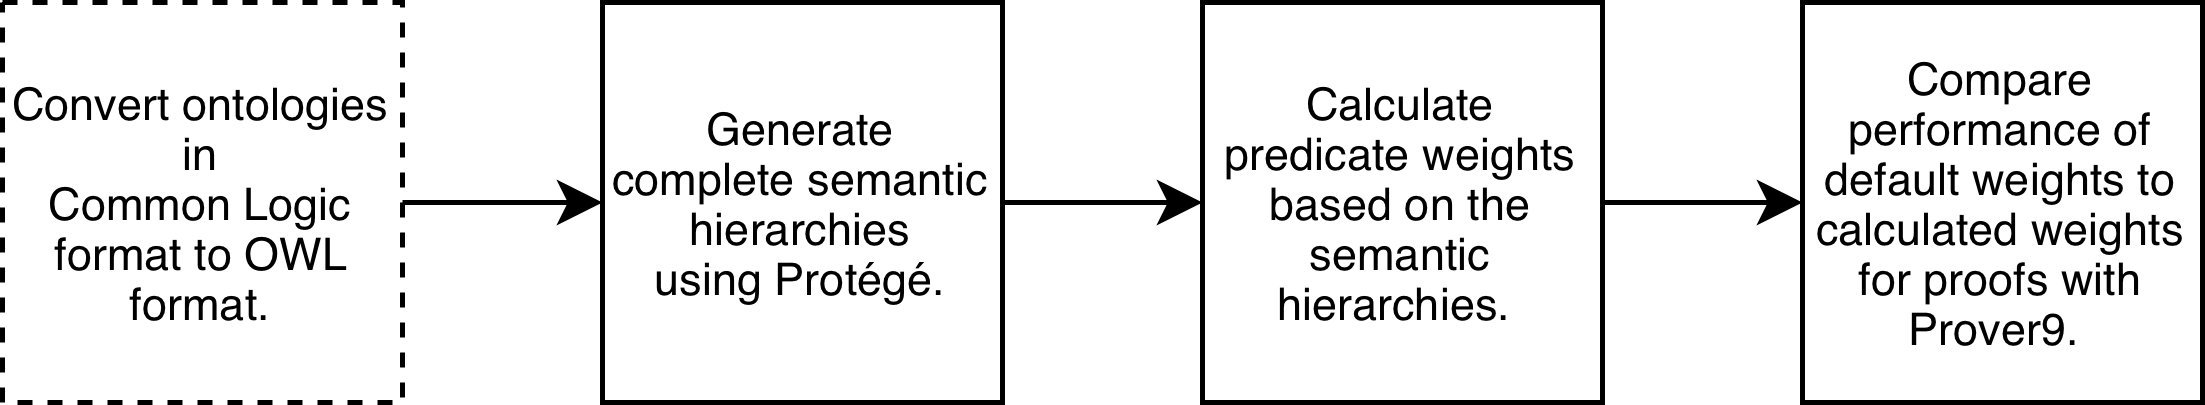
\includegraphics[width = \textwidth]{images/flowchart.png}
	}
	
		    \frame{
	    \frametitle{Functions}
	}
	
	 \frame{
	    \frametitle{Results}
	}
	
	\frame{
	    \frametitle{Limitations}
	   \texttt{(all x all y (GED(x,y) \& GED(y,x) \& (all z (CH(z,x) -> CH(z,y))) -> CS(x,y))).} 
	}
	
	
	
	    \frame{
	    \frametitle{Questions}
	}
\end{document}
